\documentclass[a4paper,11pt]{article}
\usepackage{geometry}
 \geometry{
 a4paper,
 total={170mm,257mm},
 left=20mm,
 top=20mm,
 }

 \usepackage{enumerate}
 \usepackage{amsmath}
 \usepackage{siunitx}
 \usepackage{multirow}
\usepackage{colortbl}
 \usepackage{hhline}

 \usepackage{lipsum}  %%% Lorem ipsum

\setlength{\headheight}{30.0pt}
\setlength{\footskip}{20pt}


\usepackage{hyperref}
\hypersetup{
    colorlinks=True,
    linkcolor={blue!20!black},
    filecolor=magenta,      
    urlcolor=cyan,
}



 \usepackage[export]{adjustbox}
\usepackage[english]{babel}
\usepackage[utf8]{inputenc}
\usepackage{fancyhdr}
\usepackage{multicol}

\pagestyle{fancy}
\fancyhf{}
\rhead{\textit{Pul074BEX004}}
\lhead{\textit{Amrit Prasad Phuyal}}
\rfoot{\thepage}


\usepackage{mathpazo} % Palatino font
\usepackage{graphicx}
\usepackage{float}


%%%%%% include  Titles.%%%% use \input{./CP}%%%
%%%use """"""""    \CP{}{}{}{}   """" %%%% and 4 argument to craete Title page 
%%%%%%%%%%%%%%%%%%%%%%%%%%%%%%%%%%%%%%%%%%%%%%%%%%%%%%%%%%%%%%%%%
%%%argument number
%% 1=major header ## Course name 
%% 2=minor4 heading ## lab/assignmet no
%% 3=Title  ## Assignment or Lab title
%% 4=submitted to::## input receiver Name"
%%%%%%%%%%%%%%%%%%%%%%%%%%%%%%%%%%%%%%%%%%%%%%%%%%%%%%%%%%%%%%%%%


\usepackage{mathpazo} % Palatino font
\usepackage{graphicx}
\usepackage{float}

%%% format and command for lab ans c and assembly

\newcommand{\HRule}{\rule{\linewidth}{0.4mm}} % Defines a new command for horizontal lines, change thickness here



%----------------------------------------------------------------------------------------
%	TITLE PAGE
%----------------------------------------------------------------------------------------


\newcommand{\CP}[4]{ \begin{titlepage} % Suppresses displaying the page number on the title page and the subsequent page counts as page 1
		%%%%  univerdity logo%%
		\begin{figure}[H]
			\centering
			
\includegraphics[scale=0.13]{tulogo.jpg}
		\end{figure}
		%%% end university logo

		\center % Centre everything on the page

		%------------------------------------------------
		%	Headings
		%------------------------------------------------

		\textsc{\huge Institute of Engineering \\ Central Campus,Pulchowk}\\[1.5cm] % Main heading such as the name of your university/college

		\textsc{\Large #1}\\[0.5cm] % Major heading such as course name

		\textsc{\large #2}\\[0.5cm] % Minor heading such as assignment no./ lab no.

		%------------------------------------------------
		%	Title
		%------------------------------------------------

		\HRule\\[0.4cm]

		{\Huge\bfseries #3}\\[0.4cm] % Title of your document

		\HRule\\[1.5cm]

		%------------------------------------------------
		%	Author(s)
		%------------------------------------------------
		\vfill\vfill
		\begin{minipage}{0.4\textwidth}
			\begin{flushleft}
				\large{
				\textbf{Submitted BY:}\\
				{\normalsize AMRIT PRASAD PHUYAL}\\ % NAME
				{\normalsize Roll: PULL074BEX004}} % Roll
			\end{flushleft}
		\end{minipage}
		~
		\begin{minipage}{0.4\textwidth}
			\begin{flushright}
				\large
				\textbf{Submitted To:}\\
				{ \normalsize{#4}\\ }% recepent's  Name 
				{\normalsize Department of Electronics and Computer Engineering}
			\end{flushright}
		\end{minipage}

		%------------------------------------------------
		%	Date
		%------------------------------------------------

		\vfill\vfill\vfill % Position the date 3/4 down the remaining page

		{\large\today} % Date, change the \today to a set date if you want to be precise

		\vfill % Push the date up 1/4 of the remaining page

	\end{titlepage}
} %%% cover page

%%% Formating And Command for Embedded Lab  VHDl
%% \ancode{caption}{Filename}


\usepackage{listings}
\usepackage{multicol}
\usepackage{mdframed}

\renewcommand{\lstlistlistingname}{List of MATLAB Codes}
\renewcommand{\lstlistingname}{MATLAB Code}

\setlength{\columnsep}{0.5cm}

\usepackage{xcolor}
\definecolor{codegreen}{rgb}{0,0.6,0}
\definecolor{codegray}{rgb}{0.3,0.3,0.3}
\definecolor{codepurple}{rgb}{0.58,0,0.82}
%\definecolor{backcolour}{rgb}{0.95,0.99,0.92}
\definecolor{backcolour}{rgb}{0,0,0}

\lstdefinestyle{MATLAB}{
  %backgroundcolor=\color{backcolour},  
  commentstyle=\color{codegreen},
  keywordstyle=\color{blue},
  numberstyle=\tiny\color{codegray},
  stringstyle=\color{codepurple},
  basicstyle=\ttfamily\small\color{black},
  breakatwhitespace=false,
  breaklines=true,
  captionpos=b,
  keepspaces=true,
  language=Matlab,
  numbers=left,
  numbersep=5pt,
  showspaces=false,
  frame = single,
  showstringspaces=false,
  showtabs=false,
  tabsize=3
}




\newcommand {\anscode}[2]{
  \lstinputlisting[style=MATLAB,nolol]{#2}

  \begingroup
  \captionof{lstlisting}{#1}
  \endgroup

}

%%% Formating And Command for Embedded Lab  VHDL %%% Matlab code

\newcommand\ddfrac[2]{\frac{\displaystyle #1}{\displaystyle #2}} 



%%%%%%%%%%%%%%%%%%%%%for matlab observation #1 fig name #2 Caption
\newcommand{\mobs}[2]{
    \begin{figure}[H]
        \centering
        \includegraphics[width=1.07\linewidth]{./FIG/#1.eps}
        \caption{#2}
    \end{figure}
   
}

% New command for Figure
\newcommand{\fig}[2]{
    \begin{figure}[H]
        \centering
        \includegraphics[width=0.95\linewidth]{./FIG/#1}
        \caption{#2}
    \end{figure}
}

 %%%%%%%%%%% for Python observation #1 fig name #2 Caption

\newcommand{\pobs}[2]{
    \begin{figure}[H]
        \centering
        \includegraphics[width=1.07\linewidth]{./FIG/#1.eps}
        \caption{#2}
    \end{figure}
   
}




\begin{document}


%%%%  COver page 
\CP{Digital Signal Processing}{Lab \#4}{Linear Time Invarient (LTI) system}
{Anila  Kansakar}
%%%%%%%%%%%%%%%%%%%%

\pagenumbering{gobble}
\renewcommand{\contentsname}{Table of Contents}
\tableofcontents

\pagebreak
%\listoffigures
% \pagebreak
% \vspace{5em}
\lstlistoflistings
\vspace{10em}
% \pagebreak
\listoffigures
\pagebreak
\pagenumbering{arabic}

%%%%%%%%%%%%%%%%%%%%%%%%%%%%%%%%%%%%%%%%%%%%%%
\section{Title} {\large Linear Time Invarient (LTI) system}
%%%%%%%%%%%%%%%%%%%%%%%%%%%%
\section{Objective}
\begin {itemize}
\item To understand the relationship of the frequency response of LTI system to the pole-zero of the system and its visualization.
\item To determine magnitude \& phase of transfer function and plot its zeros and poles into z-plane.
\end{itemize}
%%%%%%%%%%%%%%%%%%%%%


%Theory
\section{Theory}

\subsection{Background}
\begin{figure}[H]
    \centering
    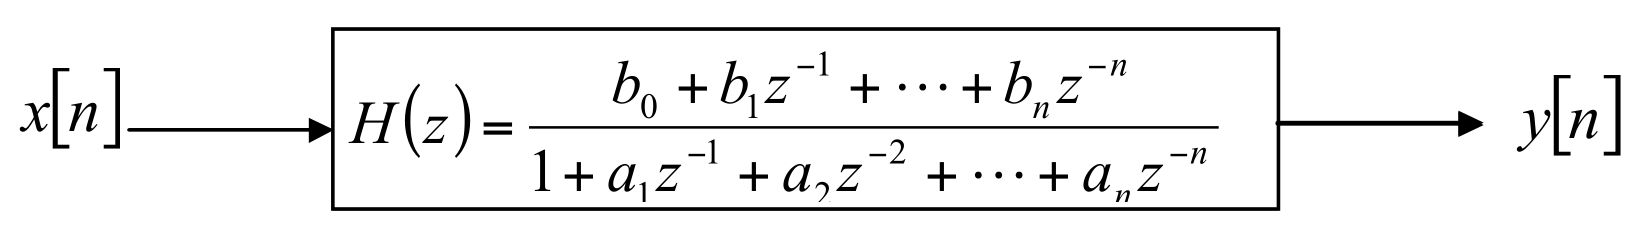
\includegraphics[width=0.8\linewidth]{./FIG/back_eq.png}
    \caption{Transfer Function of LTI system}
\end{figure}
A \textbf{linear time invariant (LTI)}system is characterized by the transfer function $H(z)=\ddfrac{Y(z)}{X(z)}$,
where $X(z)$ and $Y(z)$ are the Z-transforms of the sequences $x[n]$ and $y[n]$ respectively. When the
inverse Z-transform of the transfer function $H(z)$ is taken, the resulting difference equation can be written as:
\begin{equation*}
    y[n]=b_0x[n]+b_1x[n-1]+\dots+b_Nx[n-N]-a_1y[n-1]-a_2y[n-2]-\dots-a_Ny[n-N]
\end{equation*}
The digital signal processing basically deals with the methods of implementation of the above
difference equation. The equation can be solved using both hardware and software. It can be
implemented using microprocessor based designs in which the assembly language programming
plays the vital role. For the fast processing of the signals, considering the improved system
performance the digital signal processing chips are preferred. The DSP chips are based on the
Harvard architecture rather than the Von-Neumann's architecture, usually found in most of the
personal computers.\\

If the transfer function $H(z)$ is known for the given LTI system the MATLAB signal processing
toolbox functions can be used to plot the frequency response of the system. For this there is a
function; $[H, W]= freqz(b, a, w) $ which gives the complex values in amplitude \texttt{H} and angle \texttt{W} radians versus w points frequency. Here \texttt{a \& b} are the vector sequences representing the
numerator and denominator coefficients of $H(z)$.

\subsection{Linear Systems Transformation}
In discrete time systems the transfer function in the Z domain plays the key role in determining the nature of the system. The nature of the system is determined from the number and locations of the poles and zeros in the Z-plane. In lower order systems the locations of the poles and zeros can be easily determined from the transfer function of the system. However the higher order systems possess transfer functions with numerator and denominator polynomials of greater degree. As a result the process of determining the poles and zeros of the system becomes complex and tedious. Besides this in most of the higher order discrete time systems, the transfer function is specified in the form of second order sections. If the transfer function of the system consists of a large number of such second order sections either in cascade or parallel form, the determination of the poles and zeros of the system becomes even harder.\\

MATLAB signal processing toolbox provides a number of functions for transforming the discrete time linear systems from one form to another. The name of the functions and their purpose are listed as follows:
\begin{verbatim} 
    sos2zp >> Transforms second order sections into zeros and poles.
    sos2tf >> Performs second order sections to transfer function conversion.
    tf2zp  >> Transfer function to pole zero conversion.
    zp2sos >> Zero-poles to second order sections.
    zplane >> Plots the pole-zero diagram in Z-plane.
    freqz  >> Determines the magnitude and phase of the transfer function.
\end{verbatim}

For further information on the above functions, please refer to the MATLAB \texttt{‘help’}.


\section {Lab Problems}

%%%%%%%%%%%%Problem 1

\subsection{Problem 1}
\subsection*{In the given LTI system of fig above, if the coefficients $b$ and $a$ are specified as,\\ $b_0=0.0663,\quad b_1=0.1989,\quad b_2=0.1989,\quad b_3=0.0663$ \\$a_0=1,\quad a_1= -0.9349,\quad a_2=0.5668,\quad a_3= -0.1015$\\then the order of the system is 3 i.e. $N=3$.
    \begin{enumerate}[a.]
        \item Plot the frequency response of the system.
        \item  From the magnitude response of the system, find out the cut-off frequency.
        \item Identify the nature of the system analyzing its frequency response.
    \end{enumerate}}


\MAT{./CODES/p1.m}{Matlab code for Frequency Response of given coefficients}
\mobs{p1}{Plot of Frequency Response of given coefficients }

Response is Low pass with cutoff frequency  $0.339844 * \pi = 1.0676$ rad/sample.





%%%%%%%%%%%Problem 2

\subsection{Problem 2}
\subsection*{The transfer function of the fourth-order discrete time system is given as,
    \begin{equation*}
        H(z)=\frac{0.0018+0.0073z^{-1}+0.011z^{-2}+0.007z^{-3}+0.008z^{-4}}{1-3.0544z^{-1}+3.8291z^{-2}-2.2925z^{-3}+0.55072z^{-4}}
    \end{equation*}
    \begin{enumerate}[a.]
        \item Find out the poles and zeros of the system and plot them in the z- plane.
        \item  Use them to determine the second order sections in the cascaded form.
        \item  Plot the frequency response of the system and comment on the nature of the system.
        \item  After knowing the numerator and denominator coefficients of each second order section, draw the signal flow graph to represent the cascaded structure.
    \end{enumerate}}


\MAT{./CODES/p2.m}{Matlab code to calculate SOS \& pole-zero and visualize it }
\mobs{p2}{Plot of poles and zeros of the system along with Frequency Response }


Output of \texttt{t2sos(b,a)} is :
\begin{verbatim}
    1.0000    3.9923    4.9632    1.0000   -1.5548    0.6492
    1.0000    0.0632    0.8955    1.0000   -1.4996    0.8484
\end{verbatim}

The second order sections as determined from MATLAB are found to be:
\begin{equation*}
    H_1(z)=\ddfrac{1.0000+3.9923z^{-1}+4.9632z^{-2}}{1.0000-1.5548z^{-1}+0.6492z^{-2}}
\end{equation*}
\begin{equation*}
    H_2(z)=\ddfrac{1.0000+0.0632z^{-1}+0.8955z^{-2}}{1.0000--1.4996z^{-1}+0.8484z^{-2}}
\end{equation*}\\


The frequency response of the system is given in . The system is low pass in nature with a cutoff frequency of $0.21289\pi = 0.668813\text{rad/sample}$.

\fig{sig_flow.png}{Signal flow graph of the cascaded system}



%%%%%%%%%%%%Problem 3

\subsection{Problem 3}
\subsection*{Let a discrete time system be implemented by cascading of the following three second order sections:\\
Section 1:
$H_1(z)=\ddfrac{0.0007378(1+2z^{-1}+z^{-2})}{1-1.2686z^{-1}+0.7051z^{-2}}$\\
Section 2:
$H_2(z)=\ddfrac{1+2z^{-1}+z^{-2}}{1-1.0106z^{-1}+0.3583z^{-2}}$\\
Section 3:
$H_3(z)=\ddfrac{1+2z^{-1}+z^{-2}}{1-0.9044z^{-1}+0.2155z^{-2}}$
\begin{enumerate}[a.]
    \item Using above three second order sections in cascaded form determine the poles and zeros of the system and plot them in z-plane.
    \item Determine the transfer function of the system, formed by cascading of the above three sections. Determine the poles and zeros from this transfer function and plot them in z-plane. Your result should match with that from 3(a).
    \item Draw the direct form structures-I \& II of the system.
\end{enumerate}}

\MAT{./CODES/p3.m}{Matlab code for plotting poles and zeros of the system for given SOS}
\mobs{p3a}{Plot of poles and zeros of the cascade system }
\mobs{p3b}{Plot of poles and zeros from transfer function of the cascade system }

Output of \texttt{b} is:
\begin{verbatim} 
    0.0007    0.0044    0.0111    0.0148    0.0111    0.0044    0.0007
\end{verbatim}

Output of \texttt{a} is:
\begin{verbatim} 
    1.0000   -3.1836    4.6223   -3.7795    1.8136   -0.4800    0.0544
\end{verbatim}

\begin{equation*}
    H(z)=\frac{0.0007+0.0044z^{-1}+0.0111z^{-2}+0.0148z^{-3}+0.0111z^{-4}+0.0044z^{-5}+0.0007z^{-6}}{1-3.1836z^{-1}+4.6223z^{-2}-3.7795z^{-3}+1.8136z^{-4}-0.4800z^{-5}+0.0544z^{-6}}
\end{equation*}

\fig{d_I.png}{Direct form structure-I of the Transfer Function.}
\fig{d_II.png}{Direct form structure-II of the Transfer Function.}

%Discussion and Conclusion
\section{Discussion and Conclusion}
In this lab we familiarize ourself with Matlab and its signal processing toolbox. We have used the following functions: \texttt{sos2zp,sos2tf,tf2zp,zp2sos,zplane,freqz}.We acquire skill to find poles and zeros including second order section from Transfer function.  We also visualized linear time invariant system and its properties.

\end{document}